\documentclass[11pt]{article}
\usepackage[english]{babel}
\usepackage[utf8]{inputenc}
\usepackage{fancyhdr}
\usepackage{graphicx}

\def\Name{Ran Liao}
\def\Topic{Implementation}

\title{\textbf{\Topic}}
\author{\Name}
\markboth{Notes on \Topic\ }{Notes on \Topic\ }
\date{\today}
 
\pagestyle{fancy}
\fancyhf{}
\rhead{\date{\today} }
\lhead{Notes on \Topic\ }
\rfoot{\thepage}

\textheight=9in
%\textwidth=6.5in
\topmargin=-.75in
%\oddsidemargin=0in
%\evensidemargin=0in
 
\begin{document}
\maketitle
\noindent\makebox[\linewidth]{\rule[8pt]{5in}{0.5pt}}

\section*{Top-down Integration}

If code artifact \textit{mAbove} sends a message to artifact \textit{mBelow}, then \textit{mAbove} is implemented and integrated before \textit{mBelow}.

\begin{itemize}
	\item a, b, c, d, e, f, g, h, i, j, k, l, m (BFS order)
	\item a, b, e, h, c, d, f, i, g, j, k, l, m (Roughly DFS order)
\end{itemize}

\begin{figure}[h]
	\centering
	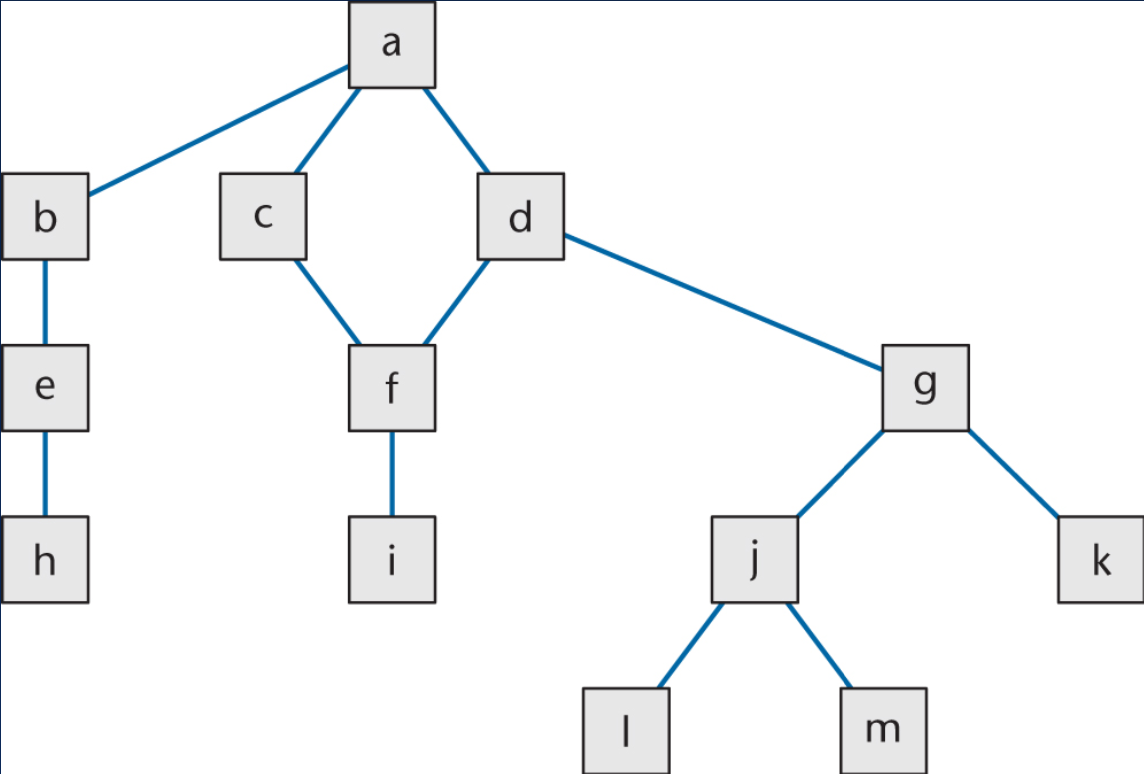
\includegraphics[width=0.6\linewidth]{images/TopDown.png}
	\caption{Artifacts Structure}
	\label{fig:TopDown}
\end{figure}

\subsection*{Advantage}

\begin{itemize}
	\item \textbf{Fault isolation}
	
	If a previously successful test case fails when \textit{mNew} is added to what has been tested so far. The fault must lie in \textit{mNew} or the interface(s) between \textit{mNew} and the rest of the product.
	
	\item \textbf{Stubs are not wasted}
	
	Each stub is expanded into the corresponding complete artifact at the appropriate step.
	
	\item \textbf{Major design flaws show up early}
	
	Logic artifacts include the decision-making flow of control. Operational artifacts perform the actual operations of the product. The logic artifacts are developed before the operational artifacts.
	
\end{itemize}

\subsection*{Disadvantage}

\begin{itemize}
	\item 
	
	Reusable artifacts are not properly tested. Lower level (operational) artifacts are not tested frequently.
	
\end{itemize}

\section*{Bottom-up Integration}

If code artifact \textit{mAbove} sends a message to artifact \textit{mBelow}, then \textit{mBelow} is implemented and integrated before \textit{mAbove}.

\begin{itemize}
	\item l, m, h, i, j, k, e, f, g, b, c, d, a
	\item h, e, b, i, f, c, l, m, j, k, g, d, a
\end{itemize}


\subsection*{Advantage}

\begin{itemize}
	\item
	
	Operational artifacts are thoroughly tested.

	\item 
	
	Operational artifacts are tested with drivers, not by fault shielding, defensively programmed artifacts.

	\item
	
	Fault isolation
	
\end{itemize}

\subsection*{Disadvantage}

\begin{itemize}
	\item 
	
	Major design faults are detected late.
	
\end{itemize}

\newpage
\section*{Sandwich Integration}

Combine top-down and bottom-up strategies making use of their strengths and minimizing their weaknesses. In Sandwich Integration, logic artifacts are integrated top-down. Operational artifacts are integrated bottom-up. Finally, the interfaces between the two groups are tested.

\begin{figure}[h]
	\centering
	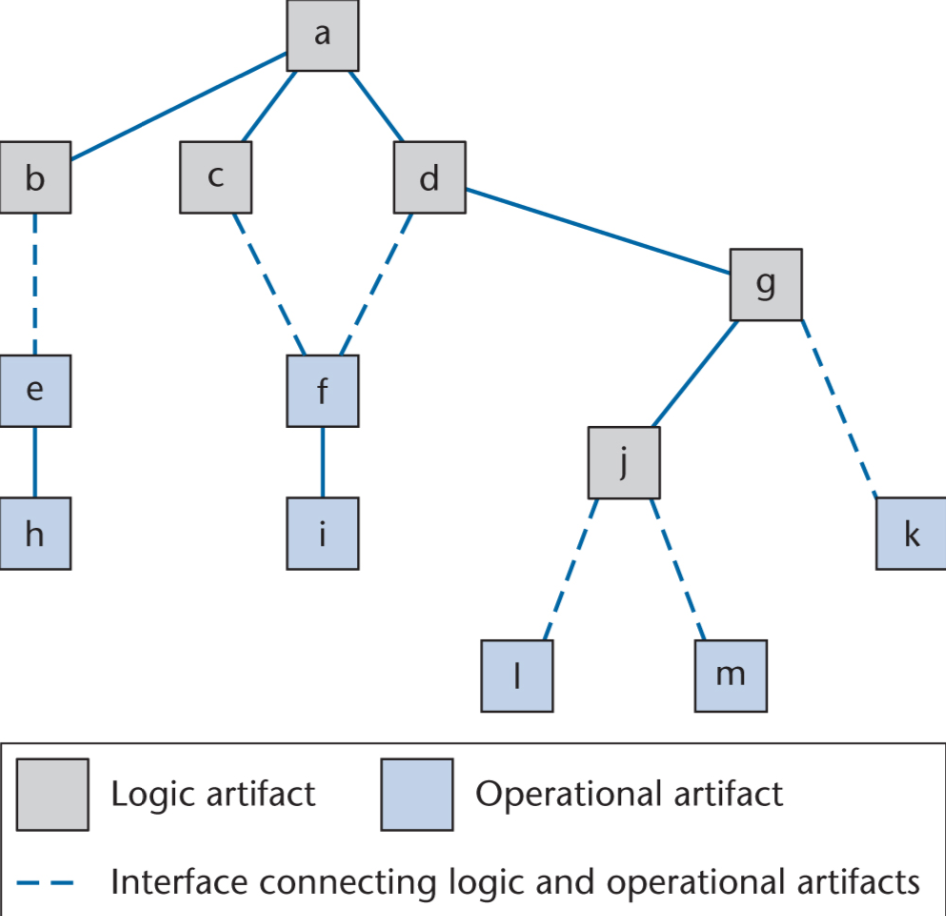
\includegraphics[width=0.6\linewidth]{images/Sandwich.png}
	\caption{Sandwich Integration}
	\label{fig:Sandwich}
\end{figure}

\subsection*{Advantage}

\begin{itemize}
	\item
	
	Major design faults are caught early

	\item 
	
	Operational artifacts are thoroughly tested.

	\item
	
	Fault isolation
	
\end{itemize}

\end{document}